\documentclass[border=10pt]{standalone}
\usepackage{pgfplots}
\pgfplotsset{compat=1.18}
\begin{document}
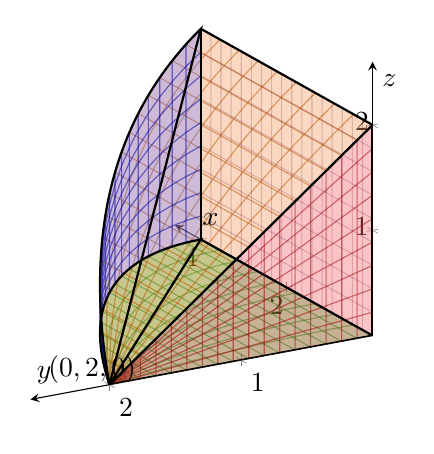
\begin{tikzpicture}
\begin{axis}[
    view={-120}{25},
    axis lines=center,
    xlabel=$x$, ylabel=$y$, zlabel=$z$,
    domain=0:2, y domain=0:1,
    samples=18, samples y=10,
    xmin=0, xmax=4.6, ymin=0, ymax=2.6, zmin=0, zmax=2.6,
    ]
% bottom
\addplot3[surf, opacity=0.32, color=green!50!black, faceted color=green!50!black, domain=0:2, y domain=0:1] ({y*(4-x^2)}, {x}, {0});
% top
\addplot3[surf, opacity=0.32, color=orange!70, faceted color=orange!70!black, domain=0:2, y domain=0:1] ({y*(4-x^2)}, {x}, {2-x});
% cylinder
\addplot3[surf, opacity=0.32, color=blue!60, faceted color=blue!60!black, domain=0:2, y domain=0:1] ({4-x^2}, {x}, {y*(2-x)});
% left wall
\addplot3[surf, opacity=0.32, color=red!60, faceted color=red!60!black, domain=0:2, y domain=0:1] ({0}, {x}, {y*(2-x)});
% back wall y=0
\addplot3[surf, opacity=0.10, color=purple!50, faceted color=purple!50!black, domain=0:4, y domain=0:1] ({x}, {0}, {y*2});
% boundary curves
\addplot3[domain=0:2, samples=100, thick, black] ({4-x^2}, {x}, {2-x});
\addplot3[domain=0:2, samples=100, thick, black] ({4-x^2}, {x}, {0});
\addplot3[domain=0:2, samples=100, thick, black] ({0}, {x}, {2-x});
\addplot3[domain=0:2, samples=100, thick, black] ({0}, {x}, {0});
\addplot3[domain=0:4, samples=100, thick, black] ({x}, {0}, {2});
\addplot3[domain=0:4, samples=100, thick, black] ({x}, {0}, {0});
\addplot3[domain=0:2, samples=100, thick, black] ({0}, {0}, {x});
\addplot3[domain=0:2, samples=100, thick, black] ({4}, {0}, {x});
\node at (axis cs:0.25,2.05,0.1) {$(0,2,0)$};
\end{axis}
\end{tikzpicture}
\end{document}